% ═══════════════════════════════════════════════════════════════════════════
%  EE2050 - FM Pocket Radio Project Report
%  Group [TBD] · Semester 3
%
%  ENGINE:   xelatex  (compile twice for TOC + refs)
%  STRUCTURE: one master preamble here; content split across part*.tex
% ═══════════════════════════════════════════════════════════════════════════
\documentclass[11pt, a4paper]{article}

% ─── Geometry & page ──────────────────────────────────────────────────────
\usepackage[margin=2.2cm, top=3.2cm, bottom=2.5cm, headheight=30pt, headsep=24pt]{geometry}
\usepackage{microtype}
\usepackage{parskip}
\usepackage{needspace}
\usepackage{etoolbox}

% Prevent widow/orphan lines and orphaned section headers
\widowpenalty=10000
\clubpenalty=10000
\displaywidowpenalty=10000
% Ensure each section/subsection pulls a few lines of body with it so the
% heading never sits alone at the bottom of a page.
\pretocmd{\section}{\needspace{6\baselineskip}}{}{}
\pretocmd{\subsection}{\needspace{5\baselineskip}}{}{}
\pretocmd{\subsubsection}{\needspace{4\baselineskip}}{}{}

% ─── Fonts (XeLaTeX) ──────────────────────────────────────────────────────
\usepackage{fontspec}
\usepackage{unicode-math}

% Body: Inter
\setmainfont{Inter}[
  UprightFont    = * Regular,
  BoldFont       = * Bold,
  ItalicFont     = * Italic,
  BoldItalicFont = * Bold Italic,
  Scale          = 0.96,
  Ligatures      = TeX
]

% Headings: Segoe UI Semibold
\newfontfamily\headingfont{Segoe UI Semibold}[
  Scale     = 0.98,
  Ligatures = TeX
]

% Monospace: Consolas
\setmonofont{Consolas}[Scale=0.88]

% Math
\setmathfont{Latin Modern Math}

% ─── Colour palette (radio-themed: teal + copper) ─────────────────────────
\usepackage{xcolor}
% Primary brand
\definecolor{brandteal}{HTML}{0F766E}     % deep teal - headings, links
\definecolor{brandcopper}{HTML}{C2410C}   % warm copper - accent rules, highlights
\definecolor{brandslate}{HTML}{475569}    % secondary accent
% Semantic
\definecolor{noteblue}{HTML}{2563EB}
\definecolor{decisiongreen}{HTML}{059669}
\definecolor{warnorange}{HTML}{EA580C}
\definecolor{failred}{HTML}{B91C1C}
\definecolor{logviolet}{HTML}{7C3AED}
% Neutrals
\definecolor{inkdark}{HTML}{0F172A}
\definecolor{inkmid}{HTML}{334155}
\definecolor{inksoft}{HTML}{64748B}
\definecolor{rulegray}{HTML}{CBD5E1}
\definecolor{zebrarow}{HTML}{F1F5F9}
\definecolor{tablehead}{HTML}{0F766E}
\definecolor{codebg}{HTML}{F8FAFC}

% ─── Graphics + tables + math ─────────────────────────────────────────────
\usepackage{graphicx}
\usepackage{amsmath}
\usepackage{booktabs}
\usepackage{array}
\usepackage{tabularx}
\usepackage{longtable}
\usepackage{multirow}
\usepackage{colortbl}
\usepackage{enumitem}
\usepackage{float}
% Allow floats to take more of the page so they don't pile at end of document
\renewcommand{\topfraction}{0.9}
\renewcommand{\bottomfraction}{0.8}
\renewcommand{\textfraction}{0.1}
\renewcommand{\floatpagefraction}{0.75}
\usepackage{caption}
\usepackage{subcaption}

\renewcommand{\arraystretch}{1.32}
\arrayrulecolor{rulegray}
\captionsetup{font={small,sf,color=inkmid}, labelfont={bf,color=brandteal}}

% Zebra-stripe tables by default (opt-in via \rowcolors)
\usepackage[table]{xcolor}

% ─── Section headings ─────────────────────────────────────────────────────
\usepackage{titlesec}

\titleformat{\section}[block]
  {\headingfont\Large\bfseries\color{brandteal}}
  {\thesection}{0.75em}{}
  [{\vspace{2pt}\color{brandcopper}\rule{2.2cm}{2.2pt}%
    \color{rulegray}\rule{\dimexpr\linewidth-2.2cm\relax}{0.4pt}}]
\titlespacing*{\section}{0pt}{1.2em}{0.6em}

\titleformat{\subsection}[block]
  {\headingfont\large\bfseries\color{brandteal!85}}
  {\thesubsection}{0.6em}{}
\titlespacing*{\subsection}{0pt}{0.9em}{0.3em}

\titleformat{\subsubsection}[block]
  {\headingfont\normalsize\bfseries\color{inkmid}}
  {\thesubsubsection}{0.5em}{}

% ─── Running header / footer ──────────────────────────────────────────────
\usepackage{fancyhdr}
\pagestyle{fancy}
\fancyhf{}
\fancyhead[L]{\small\sffamily\color{inksoft}EE2050 \textbullet{} FM Pocket Radio}
\fancyhead[R]{}
\fancyfoot[C]{\small\sffamily\color{inksoft}\thepage}
\renewcommand{\headrulewidth}{0pt}
\renewcommand{\footrulewidth}{0pt}
% Teal + copper stripe sits BELOW the header text
\renewcommand{\headrule}{%
  \vspace{6pt}\color{brandteal}\hrule height 1.2pt%
  \vspace{1pt}\color{brandcopper}\hrule height 0.5pt}

% ─── Hyperref ─────────────────────────────────────────────────────────────
\usepackage{hyperref}
\hypersetup{
  colorlinks=true,
  linkcolor=brandteal,
  urlcolor=brandteal,
  citecolor=brandteal,
  pdftitle={EE2050 - FM Pocket Radio},
  pdfauthor={Group [TBD] · University of Peradeniya}
}

% ─── Callout boxes (tcolorbox) ────────────────────────────────────────────
\usepackage[most]{tcolorbox}

\newtcolorbox{calloutnote}[1][Note]{%
  enhanced, breakable, left=10pt, right=10pt, top=6pt, bottom=6pt,
  colback=noteblue!6, colframe=noteblue!50, boxrule=0.4pt, arc=3pt,
  borderline west={3pt}{0pt}{noteblue},
  coltitle=white, colbacktitle=noteblue,
  fonttitle=\headingfont\bfseries,
  attach boxed title to top left={xshift=6pt, yshift=-2pt},
  boxed title style={arc=2pt, boxrule=0pt, left=6pt, right=6pt,
                     top=2pt, bottom=2pt},
  title=#1
}
\newtcolorbox{calloutdecision}[1][Decision]{%
  enhanced, breakable, left=10pt, right=10pt, top=6pt, bottom=6pt,
  colback=decisiongreen!6, colframe=decisiongreen!50, boxrule=0.4pt, arc=3pt,
  borderline west={3pt}{0pt}{decisiongreen},
  coltitle=white, colbacktitle=decisiongreen,
  fonttitle=\headingfont\bfseries,
  attach boxed title to top left={xshift=6pt, yshift=-2pt},
  boxed title style={arc=2pt, boxrule=0pt, left=6pt, right=6pt,
                     top=2pt, bottom=2pt},
  title=#1
}
\newtcolorbox{calloutwarn}[1][Caution]{%
  enhanced, breakable, left=10pt, right=10pt, top=6pt, bottom=6pt,
  colback=warnorange!6, colframe=warnorange!50, boxrule=0.4pt, arc=3pt,
  borderline west={3pt}{0pt}{warnorange},
  coltitle=white, colbacktitle=warnorange,
  fonttitle=\headingfont\bfseries,
  attach boxed title to top left={xshift=6pt, yshift=-2pt},
  boxed title style={arc=2pt, boxrule=0pt, left=6pt, right=6pt,
                     top=2pt, bottom=2pt},
  title=#1
}
\newtcolorbox{calloutfail}[1][Abandoned]{%
  enhanced, breakable, left=10pt, right=10pt, top=6pt, bottom=6pt,
  colback=failred!5, colframe=failred!50, boxrule=0.4pt, arc=3pt,
  borderline west={3pt}{0pt}{failred},
  coltitle=white, colbacktitle=failred,
  fonttitle=\headingfont\bfseries,
  attach boxed title to top left={xshift=6pt, yshift=-2pt},
  boxed title style={arc=2pt, boxrule=0pt, left=6pt, right=6pt,
                     top=2pt, bottom=2pt},
  title=#1
}
\newtcolorbox{logentry}[2]{%
  enhanced, breakable, left=12pt, right=10pt, top=8pt, bottom=6pt,
  colback=logviolet!5, colframe=logviolet!50, boxrule=0.4pt, arc=3pt,
  borderline west={3pt}{0pt}{logviolet},
  coltitle=white, colbacktitle=logviolet,
  fonttitle=\headingfont\bfseries\small,
  attach boxed title to top left={xshift=6pt, yshift=-2pt},
  boxed title style={arc=2pt, boxrule=0pt, left=6pt, right=6pt,
                     top=2pt, bottom=2pt},
  title={LOG ENTRY #1 \textbullet{} #2}
}

% ─── TikZ for diagrams ────────────────────────────────────────────────────
\usepackage{tikz}
\usetikzlibrary{arrows.meta, positioning, shapes.geometric, shapes.misc,
                fit, backgrounds, calc, decorations.pathreplacing}

% ─── Code listings ────────────────────────────────────────────────────────
\usepackage{listings}
\lstset{
  basicstyle=\ttfamily\small\color{inkdark},
  backgroundcolor=\color{codebg},
  frame=single,
  framerule=0.4pt,
  rulecolor=\color{rulegray},
  breaklines=true,
  columns=fullflexible,
  keepspaces=true
}

% ─── Custom helpers ───────────────────────────────────────────────────────
\newcommand{\chip}[1]{{\ttfamily\small #1}}
\newcommand{\pin}[1]{{\ttfamily\small #1}}
\newcommand{\signal}[1]{{\sffamily\small\bfseries\color{brandteal}#1}}
% Table-header row: white bold text on teal; use as \hdr{Column}
\newcommand{\hdr}[1]{{\color{white}\bfseries #1}}

% ═══════════════════════════════════════════════════════════════════════════
\begin{document}

% ══════════════════════════════════════════════════════════════════════════
%  PART 1 - Title Page, Abstract, Contents
% ══════════════════════════════════════════════════════════════════════════

% ─── Cover ────────────────────────────────────────────────────────────────
\begin{titlepage}
\thispagestyle{empty}
\begin{tikzpicture}[remember picture, overlay]
  % Full-bleed teal band at top
  \fill[brandteal] (current page.north west) rectangle
        ([yshift=-4.2cm]current page.north east);
  % Copper accent stripe
  \fill[brandcopper] ([yshift=-4.2cm]current page.north west) rectangle
        ([yshift=-4.35cm]current page.north east);
  % Geometric radio-wave pattern (concentric arcs, in top band)
  \begin{scope}
    \clip ([yshift=-0.1cm]current page.north west) rectangle
          ([yshift=-4.2cm]current page.north east);
    % Radio-wave concentric arcs emanating from left
    \foreach \r in {1.0,1.6,2.2,2.8,3.4,4.0,4.6,5.2} {
      \draw[white, opacity=0.10, line width=0.5pt]
        ([xshift=3.0cm, yshift=-2.1cm]current page.north west)
        arc[start angle=-40, end angle=40, radius=\r cm];
    }
    % Second set of arcs from right side
    \foreach \r in {1.0,1.6,2.2,2.8,3.4,4.0,4.6,5.2} {
      \draw[white, opacity=0.07, line width=0.4pt]
        ([xshift=-4.0cm, yshift=-2.1cm]current page.north east)
        arc[start angle=140, end angle=220, radius=\r cm];
    }
    % Subtle copper dots representing signal nodes
    \foreach \i in {0,1,...,12} {
      \fill[brandcopper, opacity=0.18]
        ([xshift=\i*1.7cm+1.0cm, yshift=-3.4cm]current page.north west)
        circle (2pt);
    }
  \end{scope}

  % University, top-left
  \node[anchor=north west, inner sep=0pt, text=white,
        font=\headingfont\Large\bfseries]
    at ([xshift=2.2cm, yshift=-1.2cm]current page.north west)
    {UNIVERSITY OF PERADENIYA};
  \node[anchor=north west, inner sep=0pt, text=white, opacity=0.85,
        font=\headingfont\normalsize]
    at ([xshift=2.2cm, yshift=-1.85cm]current page.north west)
    {Faculty of Engineering};
  \node[anchor=north west, inner sep=0pt, text=white, opacity=0.85,
        font=\headingfont\normalsize]
    at ([xshift=2.2cm, yshift=-2.25cm]current page.north west)
    {Department of Electrical \& Electronic Engineering};

  % Project title block, centred on page
  \node[anchor=center, text width=19cm, align=center] at
    ([yshift=1.8cm]current page.center) {%
    \headingfont\color{inkdark}
    {\fontsize{30}{36}\selectfont\bfseries Design \& Implementation of}\\[6pt]
    {\fontsize{30}{36}\selectfont\bfseries an FM Pocket Radio}\\[16pt]
    {\fontsize{15}{19}\selectfont\bfseries\color{brandcopper}%
      From Breadboard to Custom PCB}};

  % Module tag as a clean typographic element: copper rule / text / copper rule
  \node[anchor=center, font=\headingfont\small\bfseries, text=brandteal,
        inner sep=0pt]
    (modtag) at ([yshift=-0.7cm]current page.center)
    {EE2050 \hspace{0.6em}\textbullet\hspace{0.6em}
     PRODUCT DEVELOPMENT};
  \draw[brandcopper, line width=1.2pt]
    ([xshift=-8.5cm]modtag.center) -- ([xshift=-0.4cm]modtag.west);
  \draw[brandcopper, line width=1.2pt]
    ([xshift=0.4cm]modtag.east) -- ([xshift=8.5cm]modtag.center);

  % Author block with placeholder names
  \node[anchor=center, draw=rulegray, line width=0.4pt, rounded corners=6pt,
        fill=white, inner xsep=20pt, inner ysep=14pt]
    (authcard) at ([yshift=-5.0cm]current page.center) {%
    \begin{tabular}{@{}c@{}}
      \headingfont\bfseries\color{brandteal}\small Members \\[2pt]
      \color{rulegray}\rule{6cm}{0.3pt} \\[4pt]
      \ttfamily\small D.A.S.R. Dharmarathna  \\
      \ttfamily\small S.M.T.Uthpala  \\
    \end{tabular}};

  % Bottom teal rule
  \draw[brandteal, line width=2.5pt]
    ([xshift=2.2cm, yshift=0.9cm]current page.south west)
    -- ([xshift=-2.2cm, yshift=0.9cm]current page.south east);
\end{tikzpicture}
\end{titlepage}

% ─── Abstract ─────────────────────────────────────────────────────────────
\newpage
\thispagestyle{fancy}
\section*{\headingfont\color{brandteal}Abstract}
\addcontentsline{toc}{section}{Abstract}

This report documents the design, iteration, and implementation of a portable
FM pocket radio, developed across three progressive iterations for the
\textbf{EE2050 Product Development} module during Semester~3 (February to
March 2026). The project evolved through three iterations:

\begin{itemize}[leftmargin=1.8em, itemsep=2pt]
  \item \textbf{Iteration 1:} A basic Arduino UNO + RDA5807M + TDA2822M perfboard prototype.
  \item \textbf{Iteration 2:} An ESP32-based feature-rich build with OLED display and rotary encoders.
  \item \textbf{Iteration 3:} A custom PCB design featuring an ATmega328P, PAM8403 Class-D amplifier, CH340C USB-UART bridge, and single USB-C port for both charging and programming.
\end{itemize}

The design process was heavily AI-assisted, with multiple
language models consulted for circuit design, debugging, and verification.
This report captures the complete engineering journey: the problems
encountered, the solutions discovered, and the lessons learned.

% ─── Table of Contents ────────────────────────────────────────────────────
\newpage
\thispagestyle{fancy}
{\headingfont\color{brandteal}
  \renewcommand{\contentsname}{Contents}
  \tableofcontents}
\vspace{0.5cm}
\noindent\color{rulegray}\rule{\linewidth}{0.3pt}

\newpage

% ═══════════════════════════════════════════════════════════════════════════
%  Part 2 - Introduction, Objectives & Methodology
% ═══════════════════════════════════════════════════════════════════════════

\section{Introduction}

The EE2050 module requires each group to design and build a product-grade
electronic device.  This group chose to build a \textbf{pocket FM radio} - a
device that would evolve from a basic functional prototype to a professional
PCB-based product.

% ─── Problem Statement ────────────────────────────────────────────────────
\subsection{Problem Statement}

Design and build a pocket-size FM radio that:

\begin{itemize}[leftmargin=1.8em, itemsep=2pt]
  \item Receives FM broadcast (87.5–108.0\,MHz, Sri Lanka band)
  \item Provides clear audio output through both speaker and headphones
  \item Is rechargeable via USB-C
  \item Fits in a pocket ($\sim$70\,$\times$\,50\,mm PCB)
  \item Can be programmed/updated via the same USB-C port
  \item Has a user-friendly OLED display with station names
  \item Costs under Rs.\,5\,000
\end{itemize}

% ─── Project Objectives ──────────────────────────────────────────────────
\subsection{Project Objectives}

\begin{enumerate}[leftmargin=2em, itemsep=3pt]
  \item \textbf{Primary:} Build a working FM radio on perfboard (proof of
        concept)
  \item \textbf{Secondary:} Add digital UI, battery power, and encoder
        controls (feature expansion)
  \item \textbf{Tertiary:} Design a custom PCB with integrated charging,
        programming, and product-grade finish
  \item \textbf{Documentation:} Maintain a complete design log capturing
        every decision and iteration
\end{enumerate}

% ─── Key Decisions ────────────────────────────────────────────────────────
\subsection{Key Decisions}

\rowcolors{2}{zebrarow}{white}
\begin{table}[H]
\centering
\small
\begin{tabularx}{\linewidth}{>{\raggedright\arraybackslash}p{2.4cm}
                              >{\raggedright\arraybackslash}p{4.6cm}
                              >{\raggedright\arraybackslash}X}
\rowcolor{tablehead}
\hdr{Decision} & \hdr{Choice} & \hdr{Reason} \\
\midrule
MCU &
  \chip{ATmega328P-PU} (DIP-28) &
  Same as Arduino UNO, 3.3\,V / 8\,MHz, through-hole \\
Radio IC &
  \chip{RDA5807M} on RRD-102 V2.0 &
  DSP demodulation, auto-seek, I\textsuperscript{2}C, already owned \\
Amplifier &
  \chip{PAM8403} Class-D (SOP-16) &
  90\,\% efficient, $\overline{\text{SHDN}}$ mute pin, SMD \\
Display &
  \chip{SSD1306} 0.96\textquotedbl{} OLED &
  I\textsuperscript{2}C, 128\,$\times$\,64, already owned \\
Power &
  3.7\,V LiPo + \chip{HT7333} LDO &
  Low dropout ($<$100\,mV), pocket-size \\
USB &
  Single USB-C port &
  Charging (\chip{TP4056}) + programming (\chip{CH340C}) \\
Audio &
  Mono speaker + stereo headphones &
  Single speaker sufficient for pocket radio \\
\end{tabularx}
\caption{Key design decisions and rationale.}
\label{tab:key-decisions}
\end{table}
\rowcolors{1}{}{}% reset

% ─── Design Methodology ──────────────────────────────────────────────────
\subsection{Design Methodology}

\begin{enumerate}[leftmargin=2em, itemsep=2pt]
  \item \textbf{Research phase} - component selection, datasheet review,
        tutorial search
  \item \textbf{Prototype~1} - basic perfboard build; verify FM reception
        and audio
  \item \textbf{Prototype~2} - add display, encoders, battery; feature
        validation
  \item \textbf{PCB design} - custom 2-layer board in KiCad~9.0
  \item \textbf{Documentation} - comprehensive build guide + this report
\end{enumerate}

\begin{calloutdecision}[AI-Assisted Design]
Multiple AI models (ChatGPT, Gemini, Claude, Grok, DeepSeek) were consulted
throughout the project for circuit design, debugging, code generation, and
design verification.  This report documents both the benefits and pitfalls of this
approach.
\end{calloutdecision}

% ─────────────────────────────────────────────────────────────────────────────
% Part 3 - Design Evolution
% ─────────────────────────────────────────────────────────────────────────────

\section{Design Evolution}

The FM Pocket Radio project evolved through three distinct iterations, each
building on lessons learned from the previous build:
\begin{itemize}[leftmargin=1.8em, itemsep=2pt]
  \item \textbf{Iteration 1:} Proof of Concept (Perfboard)
  \item \textbf{Iteration 2:} Feature Expansion (ESP32 + OLED)
  \item \textbf{Iteration 3:} Custom PCB Design
\end{itemize}
The timeline below summarises the progression from a proof-of-concept perfboard to a custom PCB design.

%% ── Timeline Figure ─────────────────────────────────────────────────────────
\begin{figure}[htbp]
\centering
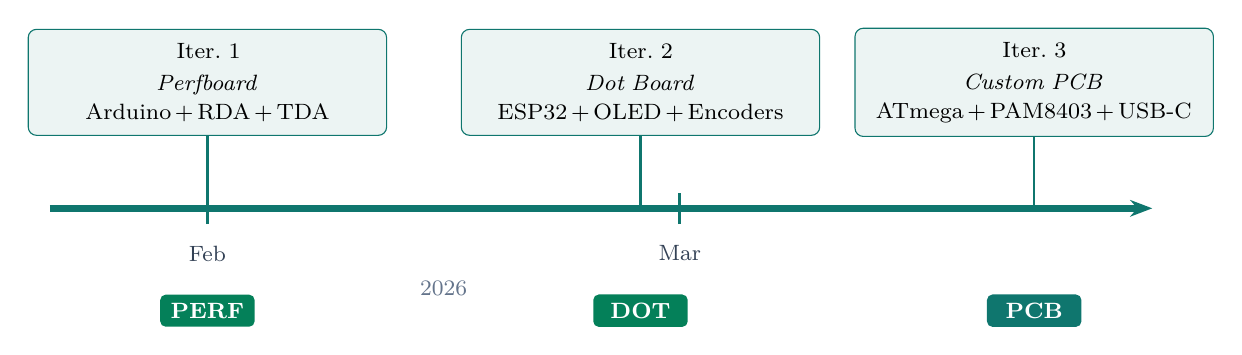
\begin{tikzpicture}[
    every node/.style={font=\small},
    iternode/.style={
        draw=brandteal, fill=brandteal!8, rounded corners=3pt,
        text width=4.2cm, align=center, font=\footnotesize\headingfont,
        inner sep=5pt
    },
    badge/.style={
        rounded corners=2pt, font=\footnotesize\bfseries,
        inner sep=3pt, minimum width=1.2cm, align=center
    }
]

% ── Backbone arrow ──
\draw[brandteal, line width=2.5pt, -{Stealth[length=8pt]}]
    (0,0) -- (14,0);

% ── Month ticks ──
\foreach \x/\lbl in {2/Feb, 8/Mar}{
    \draw[brandteal, line width=1pt] (\x,-0.2) -- (\x,0.2);
    \node[below, font=\footnotesize\headingfont, text=inkmid] at (\x,-0.35) {\lbl};
}
\node[below, font=\footnotesize, text=inksoft] at (5,-0.8) {2026};

% ── Iteration nodes ──
\node[iternode] (i1) at (2.0, 1.6)
    {Iter.\ 1\\[2pt]\textit{Perfboard}\\[1pt]Arduino\,+\,RDA\,+\,TDA};
\node[iternode] (i2) at (7.5, 1.6)
    {Iter.\ 2\\[2pt]\textit{Dot Board}\\[1pt]ESP32\,+\,OLED\,+\,Encoders};
\node[iternode] (i3) at (12.5, 1.6)
    {Iter.\ 3\\[2pt]\textit{Custom PCB}\\[1pt]ATmega\,+\,PAM8403\,+\,USB-C};

% ── Connectors ──
\draw[brandteal, thick] (i1.south) -- (2.0,0);
\draw[brandteal, thick] (i2.south) -- (7.5,0);
\draw[brandteal, thick] (i3.south) -- (12.5,0);

% ── Build-state badges ──
\node[badge, fill=decisiongreen!85!black, text=white] at (2.0,-1.3) {PERF};
\node[badge, fill=decisiongreen!85!black, text=white] at (7.5,-1.3) {DOT};
\node[badge, fill=brandteal, text=white] at (12.5,-1.3) {PCB};

\end{tikzpicture}
\caption{Design iteration timeline: February to March 2026.}
\label{fig:timeline}
\end{figure}


%% ═══════════════════════════════════════════════════════════════════════════════
\subsection{Iteration 1 - Proof of Concept (Perfboard)}
%% ═══════════════════════════════════════════════════════════════════════════════

\textbf{Period:} February 2026.

\medskip\noindent
\hdr{Components}

\begin{itemize}[nosep]
    \item \chip{Arduino UNO} (5\,V logic, ATmega328P)
    \item \chip{RDA5807M} FM receiver (\textsc{RRD-102 V2.0} module)
    \item \chip{TDA2822M} dual audio amplifier (DIP-8, single-ended mode)
    \item 4\,$\Omega$ / 5\,W speaker
    \item B100K linear volume potentiometer
    \item 2$\times$ tactile seek buttons (\signal{SEEK\_UP}, \signal{SEEK\_DOWN})
\end{itemize}

%% ── Log Entry 1 ──
\begin{logentry}{1}{Feb 17 \textbullet\ First build attempt}
Components purchased from Duino Electronics (Rs.\,230 for RDA5807M module).
Built on 15$\times$18\,cm dot board.  First power-on: no sound.  I\textsuperscript{2}C
scanner found nothing at \texttt{0x10}.  Switched to address \texttt{0x11}
(index mode) - module responded.  Then seek always stuck at 108.9\,MHz.
Discovered solder ball on 32.768\,kHz crystal cylinder preventing PLL lock.
\end{logentry}

%% ── Log Entry 2 ──
\begin{logentry}{2}{Late Feb \textbullet\ Amplifier overheating}
\chip{TDA2822M} getting extremely hot.  5\,V rail collapsing from 5\,V to
3\,V when speaker connected.  Root cause: 4\,$\Omega$ speaker at max volume
exceeds USB current capacity.  Fix: lower software volume to 12/15, add
2.2\,$\Omega$ series resistor with speaker.
\end{logentry}

%% ── Warning callout ──
\begin{calloutwarn}
\textbf{Wrong IC Purchased}: We accidentally bought \chip{TEA5767}
(\textsc{RRD-102BC}, Rs.\,550) thinking it was the same as \chip{RDA5807M}
(\textsc{RRD-102V2.0}, Rs.\,230).  Same module form factor, completely
different I\textsuperscript{2}C protocol.  Extended debugging before the
mistake was identified.
\end{calloutwarn}

\medskip\noindent
\hdr{Outcome}

Working FM radio with seek buttons and hardware volume.  Multiple revisions
(Rev~1.0 to~3.2) of the build document were produced as issues were
discovered and resolved.


%% ═══════════════════════════════════════════════════════════════════════════════
\subsection{Iteration 2 - Feature Expansion (ESP32 + OLED)}
%% ═══════════════════════════════════════════════════════════════════════════════

\textbf{Period:} Late February – March 2026.

\medskip\noindent
\hdr{Components}

\begin{itemize}[nosep]
    \item \chip{ESP32} 30-pin DevKit (dual-core, 240\,MHz)
    \item \chip{RDA5807M} FM receiver
    \item \chip{TDA2822M} amplifier (BTL mode)
    \item \chip{SH1106} 1.3\textquotedbl{}\ OLED display (128$\times$64, I\textsuperscript{2}C)
    \item 2$\times$ S141 rotary encoders (tuning + volume)
    \item 18650 Li-ion cell + \chip{TP4056} charger module
    \item 15$\times$9\,cm dot board
\end{itemize}

\medskip\noindent
\hdr{Key Changes from Iteration 1}

\begin{itemize}[nosep]
    \item BTL amplifier mode ($\approx$4$\times$ power vs.\ single-ended)
    \item Software volume via \chip{RDA5807M} register (no hardware pot)
    \item OLED display: frequency, station name, signal bars, battery\,\%, volume
    \item 68-station Sri Lankan FM database in firmware
    \item Rotary encoders for tuning and volume
    \item Battery power with voltage monitoring (100\,k/100\,k divider on \pin{GPIO34})
\end{itemize}

%% ── Decision callout ──
\begin{calloutdecision}
\textbf{BTL Mode}: Bridge-Tied Load configuration drives the speaker from
both \chip{TDA2822M} outputs (\pin{pin\,1} and \pin{pin\,3}).  Neither
speaker terminal connects to GND\@.  This delivers approximately 4$\times$
the power of single-ended mode, but grounding either speaker wire will
destroy the amplifier.
\end{calloutdecision}

%% ── Log Entry 3 ──
\begin{logentry}{3}{Late Feb \textbullet\ OLED UI development}
Full UI built with U8g2 library: \texttt{logisoso22} font for frequency,
\texttt{profont12} for labels.  Signal bars + percentage, speaker icon with
volume waves, battery icon with \%, 20-bar dancing EQ animation.  Python
Colab simulation used for rapid UI iteration without reflashing ESP32.
\end{logentry}

\medskip\noindent
\hdr{Outcome}

Feature-complete prototype with premium UX\@.  Validated all features before
PCB design.

\begin{figure}[htbp]
\centering
\begin{subfigure}{0.48\textwidth}
\centering
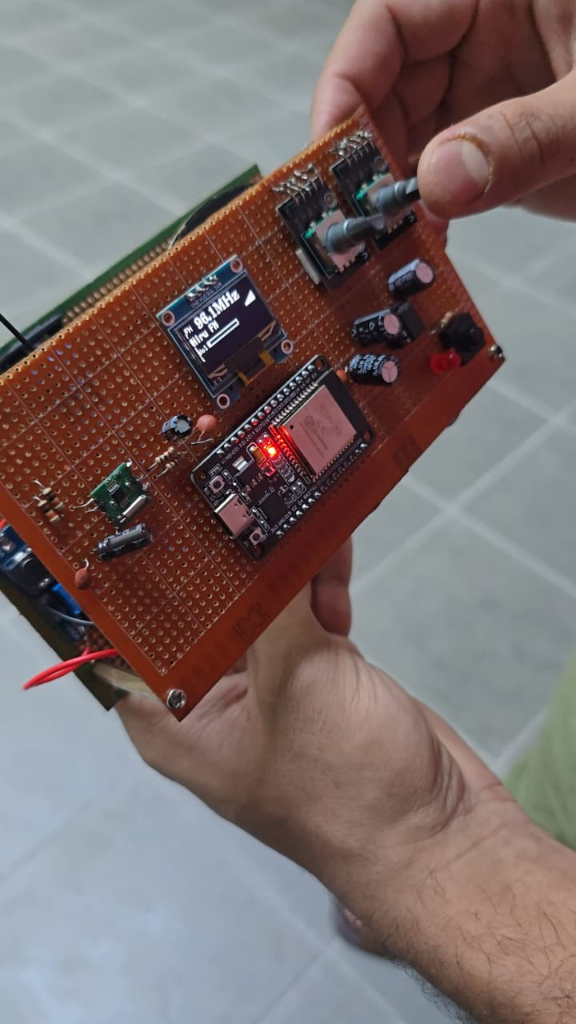
\includegraphics[width=\linewidth]{images/v2_working_1.png}
\end{subfigure}
\hfill
\begin{subfigure}{0.48\textwidth}
\centering
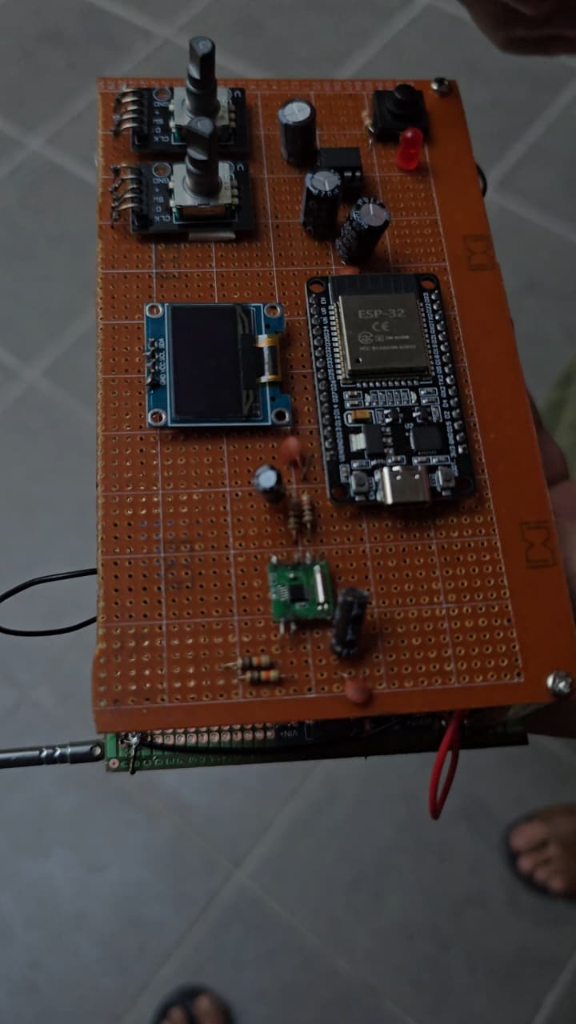
\includegraphics[width=\linewidth]{images/v2_working_2.png}
\end{subfigure}
\caption{Iteration 2 (Dot Board) physical prototype in operation.}
\label{fig:v2-prototype}
\end{figure}


%% ═══════════════════════════════════════════════════════════════════════════════
\subsection{Iteration 3 - Custom PCB Design}
%% ═══════════════════════════════════════════════════════════════════════════════

\textbf{Period:} March 2026.

\medskip\noindent
\hdr{Components}

\begin{itemize}[nosep]
    \item \chip{ATmega328P} (8\,MHz internal oscillator, 3.3\,V)
    \item \chip{RDA5807M} FM receiver
    \item \chip{PAM8403} Class-D stereo amplifier (3\,W$\times$2)
    \item \chip{CH340C} USB-to-UART bridge
    \item \chip{SSD1306} 0.96\textquotedbl{}\ OLED display (128$\times$64)
    \item \chip{TP4056} linear charger + \chip{DW01A}/\chip{FS8205A} battery protection
    \item \chip{HT7333} 3.3\,V LDO regulator
    \item USB-C connector (single port: charging + programming)
    \item Custom 70$\times$50\,mm 2-layer PCB (designed in KiCad~9.0)
\end{itemize}

\medskip\noindent
\hdr{Key Changes from Iteration 2}

\begin{itemize}[nosep]
    \item \chip{ATmega328P} replaces \chip{ESP32} (simpler, cheaper, sufficient)
    \item \chip{PAM8403} Class-D replaces \chip{TDA2822M} (90\,\% efficient, no heatsink)
    \item Single USB-C for both charging and programming
    \item On-board battery protection (\chip{DW01A} + \chip{FS8205A})
    \item Custom PCB designed in KiCad~9.0
\end{itemize}

%% ── Decision callout ──
\begin{calloutdecision}
\textbf{ATmega328P over ESP32}: For the final product, ESP32's WiFi/BT
capabilities were unnecessary overhead.  \chip{ATmega328P} at 3.3\,V /
8\,MHz provides sufficient I/O for I\textsuperscript{2}C + OLED + encoders +
ADC, runs the same Arduino ecosystem, and eliminates level-shifting
complexity.
\end{calloutdecision}

%% ── Design Status callout ──
\begin{calloutnote}[Design Status]
\textbf{Ready for Fabrication}: The Phase~3 design exists in software
(KiCad schematic + PCB layout + comprehensive build guide). It represents the \emph{target architecture}
and provides a complete foundation ready for future fabrication and assembly.
\end{calloutnote}


%% ═══════════════════════════════════════════════════════════════════════════════
\subsection{Iteration Comparison Table}
%% ═══════════════════════════════════════════════════════════════════════════════

\begin{table}[htbp]
\centering
\caption{Comparison of the three design iterations.}
\label{tab:iteration-comparison}
\small
\renewcommand{\arraystretch}{1.25}
\begin{tabularx}{\textwidth}{>{\bfseries}l X X X}
\toprule
\rowcolor{tablehead}
\textcolor{white}{\textsf{Feature}} &
\textcolor{white}{\textsf{Iter.\ 1}} &
\textcolor{white}{\textsf{Iter.\ 2}} &
\textcolor{white}{\textsf{Iter.\ 3}} \\
\midrule
\rowcolor{zebrarow}
MCU         & Arduino UNO          & ESP32                & ATmega328P \\
Radio       & RDA5807M             & RDA5807M             & RDA5807M \\
\rowcolor{zebrarow}
Amplifier   & TDA2822M (SE)        & TDA2822M (BTL)       & PAM8403 (Class-D) \\
Display     & None                 & SH1106 1.3\textquotedbl{} & SSD1306 0.96\textquotedbl{} \\
\rowcolor{zebrarow}
Volume      & Hardware pot         & Software (0--15)     & Software (0--15) \\
Tuning      & Seek buttons         & Rotary encoder       & Rotary encoder \\
\rowcolor{zebrarow}
Power       & USB 5\,V             & 18650 + TP4056       & LiPo + TP4056 + DW01A \\
Audio output& Speaker only         & Speaker only         & Speaker + headphones \\
\rowcolor{zebrarow}
Board       & 15$\times$18\,cm perfboard & 15$\times$9\,cm dot board & 70$\times$50\,mm custom PCB \\
Status      & Built \& working     & Built \& working     & Design completed \\
\bottomrule
\end{tabularx}
\end{table}

% ═══════════════════════════════════════════════════════════════════════════
%  Part 4 - System Architecture (Iteration 3 - Custom PCB)
% ═══════════════════════════════════════════════════════════════════════════

\section{System Architecture (Iteration 3)}

This section describes the complete electrical architecture of the Phase~3
custom PCB design.  Every subsystem - power, digital, RF, audio, and USB - is
integrated onto a single 2-layer FR-4 board ($\sim$70\,$\times$\,50\,mm).

% ─── Block Diagram ────────────────────────────────────────────────────────
\subsection{Block Diagram}

Figure~\ref{fig:block-diagram} shows the top-level signal and power flow.
Colour coding groups components by subsystem: \textcolor{brandcopper}{power}
(copper), \textcolor{brandteal}{digital/USB} (teal),
\textcolor{decisiongreen}{RF} (green), and
\textcolor{brandslate}{audio} (slate).

\begin{figure}[H]
\centering
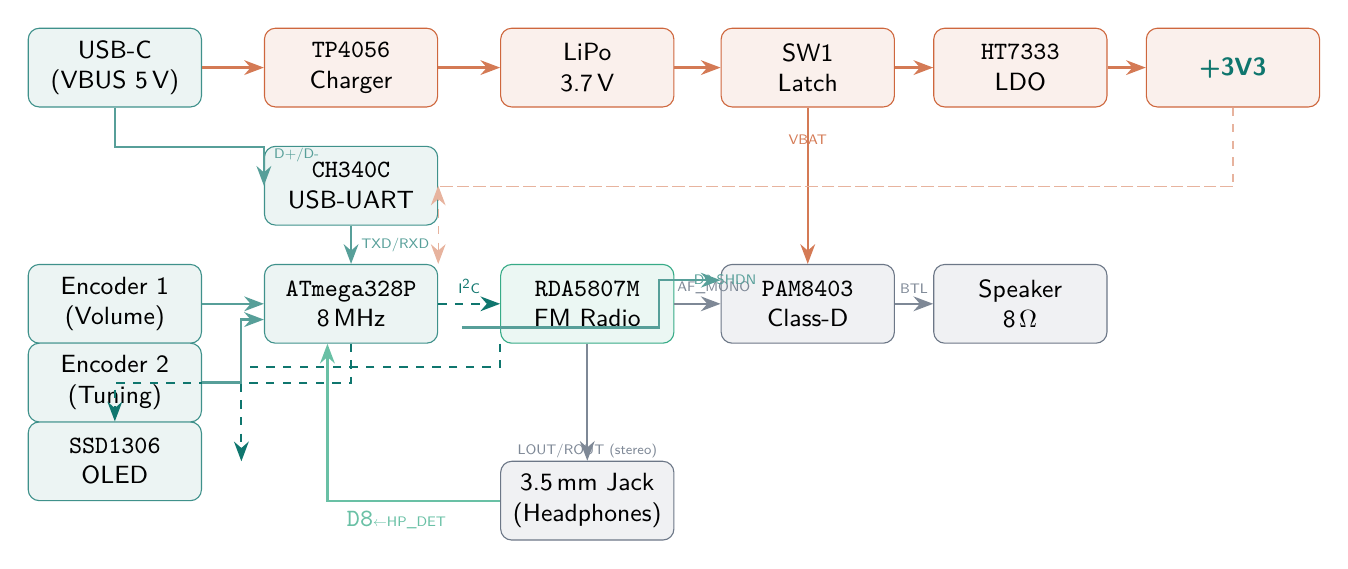
\begin{tikzpicture}[
  % ── Node styles ──
  pwr/.style  = {draw=brandcopper!80, fill=brandcopper!8, rounded corners=4pt,
                 minimum height=10mm, minimum width=22mm, align=center,
                 font=\small\sffamily},
  dig/.style  = {draw=brandteal!80, fill=brandteal!8, rounded corners=4pt,
                 minimum height=10mm, minimum width=22mm, align=center,
                 font=\small\sffamily},
  rf/.style   = {draw=decisiongreen!80, fill=decisiongreen!8, rounded corners=4pt,
                 minimum height=10mm, minimum width=22mm, align=center,
                 font=\small\sffamily},
  aud/.style  = {draw=brandslate!80, fill=brandslate!8, rounded corners=4pt,
                 minimum height=10mm, minimum width=22mm, align=center,
                 font=\small\sffamily},
  usb/.style  = {draw=brandteal!80, fill=brandteal!8, rounded corners=4pt,
                 minimum height=10mm, minimum width=22mm, align=center,
                 font=\small\sffamily},
  % ── Arrow styles ──
  pflow/.style = {-{Stealth[length=2.5mm]}, thick, brandcopper!70},
  sflow/.style = {-{Stealth[length=2.5mm]}, thick, brandteal!70},
  aflow/.style = {-{Stealth[length=2.5mm]}, thick, brandslate!70},
  rflow/.style = {-{Stealth[length=2.5mm]}, thick, decisiongreen!70},
  bus/.style   = {-{Stealth[length=2.5mm]}, thick, brandteal, dashed},
]

% ── Power chain (top row) ──
\node[usb]  (usbc)    at (0,0)     {USB-C\\(VBUS 5\,V)};
\node[pwr]  (tp4056)  at (3,0)     {\chip{TP4056}\\Charger};
\node[pwr]  (lipo)    at (6,0)     {LiPo\\3.7\,V};
\node[pwr]  (sw1)     at (8.8,0)   {SW1\\Latch};
\node[pwr]  (ldo)     at (11.5,0)  {\chip{HT7333}\\LDO};
\node[pwr]  (v33)     at (14.2,0)  {\signal{+3V3}};

% Power arrows
\draw[pflow] (usbc)   -- (tp4056);
\draw[pflow] (tp4056) -- (lipo);
\draw[pflow] (lipo)   -- (sw1);
\draw[pflow] (sw1)    -- (ldo);
\draw[pflow] (ldo)    -- (v33);

% ── VBAT direct to PAM8403 ──
\node[aud]  (pam)     at (8.8,-3)  {\chip{PAM8403}\\Class-D};
\draw[pflow] (sw1.south) -- ++(0,-0.6) -| node[pos=0.25, above, font=\tiny\sffamily\color{brandcopper}] {VBAT} (pam.north);

% ── Digital subsystem (middle row) ──
\node[dig]  (mcu)     at (3,-3)    {\chip{ATmega328P}\\8\,MHz};
\node[dig]  (oled)    at (0,-5)    {\chip{SSD1306}\\OLED};
\node[dig]  (enc1)    at (0,-3)    {Encoder~1\\(Volume)};
\node[dig]  (enc2)    at (0,-4)    {Encoder~2\\(Tuning)};

% ── RF subsystem ──
\node[rf]   (rda)     at (6,-3)    {\chip{RDA5807M}\\FM Radio};

% ── Audio output ──
\node[aud]  (spk)     at (11.5,-3) {Speaker\\8\,$\Omega$};
\node[aud]  (jack)    at (6,-5.5)  {3.5\,mm Jack\\(Headphones)};

% ── USB/UART ──
\node[usb]  (ch340)   at (3,-1.5)  {\chip{CH340C}\\USB-UART};

% ── I2C bus ──
\draw[bus] (mcu.east) -- node[above, font=\tiny\sffamily\color{brandteal}] {I\textsuperscript{2}C} (rda.west);
\draw[bus] (mcu.south) -- ++(0,-0.5) -| (oled.north);
\draw[bus] (rda.south west) -- ++(0,-0.3) -| ([xshift=5mm]oled.east);

% ── Audio paths ──
\draw[aflow] (rda.south) -- ++(0,-0.8) -- node[below, font=\tiny\sffamily\color{brandslate}] {LOUT/ROUT (stereo)} (jack.north);
\draw[aflow] (rda.east) -- ++(0.5,0) |- node[pos=0.3, above, font=\tiny\sffamily\color{brandslate}] {AF\_MONO} (pam.west);
\draw[aflow] (pam.east) -- node[above, font=\tiny\sffamily\color{brandslate}] {BTL} (spk.west);

% ── Mute control ──
\draw[sflow] (mcu.east) ++(0.3,-0.3) -- ++(2.5,0) |- node[pos=0.7, right, font=\tiny\sffamily\color{brandteal}] {D9 SHDN} ([yshift=3mm]pam.west);

% ── HP detect ──
\draw[sflow, decisiongreen!60] (jack.west) -| node[pos=0.3, below, font=\tiny\sffamily\color{decisiongreen}] {\pin{D8}$\leftarrow$HP\_DET} ([xshift=-3mm]mcu.south);

% ── USB data ──
\draw[sflow] (usbc.south) -- ++(0,-0.5) -| node[pos=0.6, right, font=\tiny\sffamily\color{brandteal}] {D+/D-} (ch340.west);
\draw[sflow] (ch340.south) -- node[right, font=\tiny\sffamily\color{brandteal}] {TXD/RXD} (mcu.north);

% ── Encoders ──
\draw[sflow] (enc1.east) -- (mcu.west |- enc1.east);
\draw[sflow] (enc2.east) -- ++(0.5,0) |- ([yshift=-2mm]mcu.west);

% ── +3V3 distribution (light dashed) ──
\draw[pflow, dashed, thin, brandcopper!40]
  (v33.south) -- ++(0,-1) -| (mcu.north east);
\draw[pflow, dashed, thin, brandcopper!40]
  (v33.south) ++(0,-1) -| (ch340.east);

\end{tikzpicture}
\caption{Phase~3 system block diagram.  Dashed lines = I\textsuperscript{2}C bus;
         solid arrows = power/signal flow.}
\label{fig:block-diagram}
\end{figure}

% ─── Power Architecture ──────────────────────────────────────────────────
\subsection{Power Architecture}

The power system is designed around a single-cell 3.7\,V LiPo (800–1000\,mAh)
with on-board charging, protection, and regulation.

\subsubsection{Charging}

USB-C VBUS (5\,V) feeds the \chip{TP4056} linear charger.  The charge current
is set by \pin{PROG} resistor R9:
%
\[
  I_{\text{charge}} = \frac{1000\,\text{V}}{R_9}
                    = \frac{1000}{2200} \approx 455\,\text{mA}
\]
%
The \chip{TP4056} implements CC/CV charging: constant current at 455\,mA until
the cell reaches 4.2\,V, then constant voltage until current tapers to
$\sim$45\,mA (1/10 termination).

\subsubsection{Battery Protection}

The LiPo \pin{BAT-} terminal connects through a \chip{DW01A} + \chip{FS8205A}
low-side protection circuit.  Two back-to-back N-channel MOSFETs
(\chip{FS8205A}) sit in the ground return path:
%
\begin{itemize}[leftmargin=1.8em, itemsep=2pt]
  \item \textbf{Over-discharge:} \chip{DW01A} opens the discharge FET when
        $V_{\text{cell}} < 2.4$\,V
  \item \textbf{Over-charge:} opens the charge FET above 4.3\,V (backup to
        \chip{TP4056})
  \item \textbf{Short-circuit:} opens within $\sim$10\,ms if current exceeds
        $\sim$3\,A
\end{itemize}

\subsubsection{Regulation}

VBAT (3.0–4.2\,V) passes through latching switch SW1, then enters the
\chip{HT7333} LDO which outputs a stable \signal{+3V3} rail.  This rail powers:
%
\begin{itemize}[leftmargin=1.8em, itemsep=2pt]
  \item \chip{ATmega328P} (MCU)
  \item \chip{RDA5807M} (FM radio)
  \item \chip{SSD1306} OLED module
  \item 2$\times$ rotary encoders (pull-ups)
  \item \chip{CH340C} (USB-UART bridge)
\end{itemize}

\subsubsection{Audio Power}

The \chip{PAM8403} amplifier is powered \emph{directly} from VBAT (post-switch),
bypassing the LDO.  This maximises available audio power:
%
\[
  P_{\text{spk}} = \frac{V_{\text{BAT}}^2}{2 \cdot R_L}
                 = \frac{4.2^2}{2 \times 8} \approx 1.1\,\text{W (peak)},
  \quad \text{typical} \approx 0.5\,\text{W}
\]
%
Running the amplifier from the unregulated rail also avoids injecting Class-D
switching noise into the sensitive 3.3\,V digital/RF supply.

\subsubsection{Battery Sensing}

VBAT is divided by R7/R8 (100\,k$\Omega$ / 100\,k$\Omega$) and filtered by
C19 (100\,nF) before reaching \pin{A0} on the \chip{ATmega328P}:
%
\[
  V_{A0} = V_{\text{BAT}} \times \frac{100\text{k}}{100\text{k}+100\text{k}}
         = \frac{V_{\text{BAT}}}{2}
\]
%
At full charge (4.2\,V), $V_{A0} = 2.1$\,V; at cutoff (3.0\,V),
$V_{A0} = 1.5$\,V.  The 100\,nF capacitor compensates for the high source
impedance (50\,k$\Omega$ Thévenin) which exceeds the ATmega's recommended
$\leq$10\,k$\Omega$ for accurate ADC sampling.

\begin{calloutnote}[HT7333 vs AMS1117 - Why Dropout Matters]
At battery minimum (3.0\,V), the \chip{HT7333} outputs $\sim$2.9\,V (dropout
$<$100\,mV).  The \chip{ATmega328P} runs reliably at 2.9\,V / 8\,MHz - its
minimum operating voltage is 2.4\,V at this frequency.  The commonly-used
\chip{AMS1117-3.3} requires $\geq$1\,V headroom and would fail below 4.3\,V
battery - completely unsuitable for a single-cell LiPo design.
\end{calloutnote}

% ─── Audio Signal Path ────────────────────────────────────────────────────
\subsection{Audio Signal Path}

\subsubsection{Mono Speaker Path}

The \chip{RDA5807M} provides stereo line-level outputs (\pin{LOUT}, \pin{ROUT}).
These are passively mixed to mono:
%
\begin{center}
\small
\pin{LOUT} $\xrightarrow{\text{R3 (10\,k}\Omega\text{)}}$
\signal{AF\_MONO}
$\xleftarrow{\text{R4 (10\,k}\Omega\text{)}}$ \pin{ROUT}
\end{center}
%
The mixed signal passes through C5 (1\,$\mu$F DC-blocking capacitor) into
\chip{PAM8403} \pin{INL}.  The amplifier drives the speaker in Bridge-Tied Load
(BTL) configuration via \pin{OUTL+} and \pin{OUTL-}, delivering up to
$\sim$0.5\,W into 8\,$\Omega$.

\subsubsection{Stereo Headphone Path}

For headphone output, the \chip{RDA5807M} outputs are AC-coupled directly to
the 3.5\,mm jack:
%
\begin{itemize}[leftmargin=1.8em, itemsep=2pt]
  \item \pin{LOUT} $\to$ C6 (10\,$\mu$F) $\to$ Jack TIP (left)
  \item \pin{ROUT} $\to$ C7 (10\,$\mu$F) $\to$ Jack RING (right)
\end{itemize}
%
The 10\,$\mu$F coupling capacitors set a $-$3\,dB low-frequency corner of:
%
\[
  f_c = \frac{1}{2\pi \cdot C \cdot R_{\text{load}}}
      = \frac{1}{2\pi \times 10\,\mu\text{F} \times 32\,\Omega}
      \approx 500\,\text{Hz (acceptable for FM audio)}
\]

\subsubsection{Antenna Coupling}

The headphone cable doubles as the FM antenna.  A 100\,pF capacitor (C8)
AC-couples the Jack TIP to the \chip{RDA5807M} \pin{ANT} pin:
%
\begin{itemize}[leftmargin=1.8em, itemsep=2pt]
  \item C8 passes RF ($>$87\,MHz) while blocking audio frequencies
  \item The headphone wire acts as a $\sim$75\,cm monopole antenna
  \item No external antenna is needed when headphones are plugged in
\end{itemize}

\subsubsection{Mute Logic}

Headphone insertion is detected by the PJ-320A jack's internal switch on
\pin{D8}:
%
\begin{enumerate}[leftmargin=2em, itemsep=2pt]
  \item Plug inserted $\to$ \pin{D8} state changes (HP\_DETECT)
  \item Firmware pulls \pin{D9} LOW
  \item \pin{D9} drives \chip{PAM8403} $\overline{\text{SHDN}}$ LOW $\to$ amplifier
        enters shutdown
  \item Speaker mutes; audio continues through headphones only
\end{enumerate}

\subsubsection{Volume Control}

Volume is controlled digitally via the \chip{RDA5807M} register \texttt{0x05},
bits [3:0].  Range: 0 (mute) to 15 (maximum).  No analogue potentiometer is
used - the left rotary encoder adjusts this register in firmware.

% ─── USB-C Integration ────────────────────────────────────────────────────
\subsection{USB-C Integration}

A single USB-C receptacle serves both charging and programming - no separate
power jack or FTDI cable required.

\subsubsection{Pin Allocation}

\begin{itemize}[leftmargin=1.8em, itemsep=2pt]
  \item \textbf{VBUS (5\,V)} $\to$ \chip{TP4056} \pin{IN+} for battery charging
  \item \textbf{D+ / D-} $\to$ \chip{CH340C} for USB-to-UART conversion
  \item \textbf{CC1 / CC2} $\to$ 5.1\,k$\Omega$ pull-downs to GND (USB-C device
        identification per USB Type-C specification)
\end{itemize}

\subsubsection{UART Bridge}

The \chip{CH340C} converts USB data to 3.3\,V UART:
%
\begin{itemize}[leftmargin=1.8em, itemsep=2pt]
  \item \chip{CH340C} \pin{TXD} $\to$ \chip{ATmega328P} \pin{RXD} (PD0)
  \item \chip{CH340C} \pin{RXD} $\leftarrow$ \chip{ATmega328P} \pin{TXD} (PD1)
\end{itemize}

\subsubsection{Auto-Reset}

The Arduino-standard auto-reset circuit allows the IDE to reset the MCU before
upload:
%
\begin{center}
\small
\chip{CH340C} \pin{DTR\#} $\to$ C14 (100\,nF) $\to$ \chip{ATmega328P}
\pin{RESET}
\end{center}
%
The capacitor differentiates the DTR edge into a brief reset pulse ($\sim$1\,ms)
without holding RESET permanently low.

\subsubsection{3.3\,V Operation (V3 Pin)}

The \chip{CH340C} \pin{V3} (pin~4) \textbf{must} be tied to VCC for 3.3\,V I/O
level operation.  A 100\,nF bypass capacitor (C18) is placed between \pin{V3}
and GND.  This configures the internal voltage regulator to output 3.3\,V on
the data lines.

\begin{calloutwarn}[Power Switch Must Be ON for USB]
The \chip{CH340C} is powered from the \signal{+3V3} rail, which is downstream
of the latching power switch SW1.  If SW1 is OFF, the \chip{CH340C} has no
power and the USB-C port appears completely dead to the host PC - no COM port
enumerates.  \textbf{The radio must be turned ON before attempting firmware
upload.}
\end{calloutwarn}

% ─── Complete BOM ─────────────────────────────────────────────────────────
\subsection{Complete Bill of Materials}

Table~\ref{tab:bom} lists every component on the Phase~3 PCB.

\rowcolors{2}{zebrarow}{white}
\begin{longtable}{
  >{\ttfamily\small}l
  >{\raggedright\arraybackslash\small}p{3.2cm}
  >{\raggedright\arraybackslash\small}p{2.8cm}
  >{\small}c
  >{\small}c
  >{\raggedright\arraybackslash\small}p{3.8cm}
}
\caption{Phase~3 complete bill of materials.}
\label{tab:bom} \\

\rowcolor{tablehead}
\hdr{Ref} & \hdr{Component} & \hdr{Value / Part} & \hdr{Pkg} & \hdr{Qty} & \hdr{Purpose} \\
\midrule
\endfirsthead

\rowcolor{tablehead}
\hdr{Ref} & \hdr{Component} & \hdr{Value / Part} & \hdr{Pkg} & \hdr{Qty} & \hdr{Purpose} \\
\midrule
\endhead

\midrule
\multicolumn{6}{r}{\small\itshape Continued on next page\ldots} \\
\endfoot

\bottomrule
\endlastfoot

% ── ICs ──
\rowcolor{tablehead!15}
\multicolumn{6}{l}{\textbf{\color{brandteal}Integrated Circuits}} \\
U1 & Microcontroller & ATmega328P-PU & DIP-28 & 1 & Main MCU (8\,MHz, 3.3\,V) \\
U2 & FM Radio Module & RDA5807M (RRD-102) & Module & 1 & DSP FM receiver, I\textsuperscript{2}C \\
U3 & Audio Amplifier & PAM8403 & SOP-16 & 1 & Class-D, mono BTL to speaker \\
U4 & LiPo Charger & TP4056 & SOP-8 & 1 & CC/CV charger, 455\,mA \\
U5 & LDO Regulator & HT7333 & SOT-89 & 1 & 3.3\,V, $<$100\,mV dropout \\
U6 & USB-UART Bridge & CH340C & SOP-16 & 1 & USB-to-serial, 3.3\,V \\
U7 & Battery Protect IC & DW01A & SOT-23 & 1 & OVP / UVP / OCP control \\
Q1 & Dual N-FET & FS8205A & SOT-23-6 & 1 & Low-side protection switches \\
  & OLED Display & SSD1306 128$\times$64 & Module & 1 & 0.96\textquotedbl{} I\textsuperscript{2}C display \\

% ── Resistors ──
\rowcolor{tablehead!15}
\multicolumn{6}{l}{\textbf{\color{brandteal}Resistors}} \\
R1, R2 & Pull-up & 4.7\,k$\Omega$ & 0805 & 2 & I\textsuperscript{2}C bus (SDA, SCL) \\
R3, R4 & Mixing & 10\,k$\Omega$ & 0805 & 2 & L+R mono summing network \\
R5 & Pull-up & 10\,k$\Omega$ & 0805 & 1 & RESET pull-up \\
R6 & Current limit & 330\,$\Omega$ & 0805 & 1 & Power LED \\
R7, R8 & Divider & 100\,k$\Omega$ & 0805 & 2 & Battery voltage sensing \\
R9 & PROG & 2.2\,k$\Omega$ & 0805 & 1 & TP4056 charge current (455\,mA) \\
R10, R11 & Pull-down & 5.1\,k$\Omega$ & 0805 & 2 & USB-C CC1/CC2 \\
R12, R13 & Current limit & 1\,k$\Omega$ & 0805 & 2 & CHRG/STDBY LEDs \\
R14 & Sense & 100\,$\Omega$ & 0805 & 1 & DW01A current sense \\

% ── Capacitors ──
\rowcolor{tablehead!15}
\multicolumn{6}{l}{\textbf{\color{brandteal}Capacitors}} \\
C1, C2 & Bypass & 100\,nF & 0805 & 2 & ATmega328P VCC/AVCC \\
C3 & Load & 22\,pF $\times$2 & 0805 & 2 & Crystal load capacitors \\
C4 & Bypass & 100\,nF & 0805 & 1 & RDA5807M supply \\
C5 & Coupling & 1\,$\mu$F & 0805 & 1 & Audio DC block (mono path) \\
C6, C7 & Coupling & 10\,$\mu$F & 0805 & 2 & Headphone DC block (L, R) \\
C8 & Antenna & 100\,pF & 0805 & 1 & RF coupling to jack \\
C9, C10 & Filter & 10\,$\mu$F & 0805 & 2 & HT7333 input/output \\
C11 & Bypass & 10\,$\mu$F & 0805 & 1 & PAM8403 PVCC (ch.~1) \\
C12 & Filter & 10\,$\mu$F & 0805 & 1 & TP4056 input \\
C13 & Bypass & 100\,nF & 0805 & 1 & CH340C VCC \\
C14 & Auto-reset & 100\,nF & 0805 & 1 & DTR\# to RESET \\
C15 & Filter & 1\,$\mu$F & 0805 & 1 & TP4056 output \\
C16 & Bulk & 10\,$\mu$F & 0805 & 1 & RDA5807M bulk decoupling \\
C17 & Filter & 1\,$\mu$F & 0805 & 1 & TP4056 BAT pin \\
C18 & Bypass & 100\,nF & 0805 & 1 & CH340C V3 pin \\
C19 & Filter & 100\,nF & 0805 & 1 & ADC input (A0) \\
C20 & Bypass & 10\,$\mu$F & 0805 & 1 & PAM8403 PVCC (ch.~2) \\
C21 & Reference & 100\,nF & 0805 & 1 & ATmega AREF stability \\

% ── Connectors & Mechanical ──
\rowcolor{tablehead!15}
\multicolumn{6}{l}{\textbf{\color{brandteal}Connectors \& Mechanical}} \\
J1 & Audio Jack & PJ-320A & TH & 1 & 3.5\,mm stereo + HP detect \\
J2 & Battery & JST PH 2-pin & TH & 1 & LiPo connection \\
J3 & ISP Header & 2$\times$3 pin (2.54\,mm) & TH & 1 & Bootloader / ISP programming \\
J4 & USB-C & 16-pin receptacle & SMD & 1 & Charging + data \\
J5 & OLED Header & 4-pin (2.54\,mm) & TH & 1 & GND-VCC-SCL-SDA \\
J6, J7 & Encoder Headers & 5-pin (2.54\,mm) & TH & 2 & Rotary encoder connection \\
J8 & Radio Module & 10-pin (1.27\,mm) & TH & 1 & RDA5807M module socket \\
J9 & Speaker & 2-pin (2.54\,mm) & TH & 1 & Speaker connection \\
SW1 & Power Switch & Latching push & TH & 1 & Main power on/off \\
Y1 & Crystal & 8\,MHz & HC-49S & 1 & MCU clock source \\

\end{longtable}
\rowcolors{1}{}{}% reset zebra

% ═══════════════════════════════════════════════════════════════════════════
%  Part 5 - PCB Design & KiCad Workflow
% ═══════════════════════════════════════════════════════════════════════════

\section{PCB Design \& KiCad Workflow}

This section documents the complete PCB design process - from tool selection
and library creation through schematic entry, layout, and DRC resolution.
The workflow reflects our realities as first-time KiCad users inheriting an
incomplete project from a teammate.

% ─── Design Tool Selection ────────────────────────────────────────────────
\subsection{Design Tool Selection}

KiCad~9.0 was chosen as the EDA tool for the following reasons:

\begin{itemize}[leftmargin=1.8em, itemsep=2pt]
  \item \textbf{Free and open-source} - no licence cost or seat restrictions
  \item \textbf{University standard} - recommended by the department for
        coursework submissions
  \item \textbf{Full-featured} - schematic capture, PCB layout, 3D viewer,
        Gerber export, and DRC in a single package
\end{itemize}


% ─── Custom Symbol & Footprint Creation ──────────────────────────────────
\subsection{Custom Symbol \& Footprint Creation}

Several components on the Phase~3 board have no standard KiCad library parts.
Custom symbols and/or footprints were created for each:

\begin{itemize}[leftmargin=1.8em, itemsep=2pt]
  \item \chip{RDA5807M} module - 11$\times$11\,mm, 2$\times$5 pads,
        1.27\,mm pitch (castellation footprint, no standard library match)
  \item \chip{PAM8403} (SOP-16) - custom symbol with correct pin mapping
  \item \chip{TP4056} (SOP-8) - custom symbol
  \item \chip{CH340C} (SOP-16) - custom symbol
  \item \chip{HT7333} (SOT-89) - custom symbol
  \item \chip{FS8205A} (SOT-23-6) - custom symbol
\end{itemize}

\begin{logentry}{4}{Feb 17 \textbullet{} Custom RDA5807M symbol}
First attempt at creating a custom KiCad symbol for the \chip{RDA5807M} module.
Made critical errors: used wrong pin types (all set to \texttt{Passive} instead
of \texttt{Bidirectional} for SDA/SCL, \texttt{Power I/O} for VCC/GND,
\texttt{Output} for LOUT/ROUT).  Also had no pin numbers - only names.  KiCad
couldn't match symbol pins to footprint pads.  Required complete rebuild of the
symbol.
\end{logentry}

% ─── Library Path Issues ─────────────────────────────────────────────────
\subsection{Library Path Issues}

\begin{calloutwarn}[Library Path Hell]
The KiCad project referenced the teammate's old PC paths
(\texttt{C:\textbackslash Users\textbackslash OtherUser\textbackslash\ldots})
in \texttt{fp-lib-table} and \texttt{sym-lib-table}.  Every footprint showed
\emph{``not found''}.  Fix: replace all absolute paths with
\texttt{\$\{KIPRJMOD\}} variable for portability.  Also discovered the
\chip{TP4056} entry was pointing to the \chip{PAM8403} folder due to a
copy-paste error.
\end{calloutwarn}

% ─── Schematic Entry ─────────────────────────────────────────────────────
\subsection{Schematic Entry}

After resolving library paths and rebuilding custom symbols, the schematic was
entered and validated using KiCad's Electrical Rules Check (ERC).

\subsubsection{ERC Results}

\begin{itemize}[leftmargin=1.8em, itemsep=2pt]
  \item \textbf{Initial run:} 1~error + 18~warnings
  \item \textbf{Fixed:} \texttt{power\_pin\_not\_driven} error - a power flag
        was missing on the battery net
  \item \textbf{Remaining warnings:} bidirectional pin conflicts
        (\chip{PAM8403} symbol pin types), unconnected pins (acceptable -
        unused MCU I/O)
  \item \textbf{Final ERC:} 0~errors, 4~warnings (SW1/SW2 mechanical pads -
        ignorable)
\end{itemize}

% ─── PCB Layout ──────────────────────────────────────────────────────────
\subsection{PCB Layout}

\subsubsection{Board Outline \& Mechanical}

\begin{itemize}[leftmargin=1.8em, itemsep=2pt]
  \item Board dimensions: 70\,$\times$\,50\,mm rectangle
  \item Corner treatment: 2\,mm fillet (rounded corners)
  \item Mounting: M3 holes at all four corners
\end{itemize}

\subsubsection{Design Rules}

\begin{itemize}[leftmargin=1.8em, itemsep=2pt]
  \item Minimum trace width: 0.25\,mm (signal traces)
  \item Power traces: 0.5–1.0\,mm (VBAT, +3V3 distribution)
  \item Clearance: 0.2\,mm minimum copper-to-copper
  \item Via drill: 0.3\,mm
\end{itemize}

\subsubsection{Layer Stackup}

\begin{itemize}[leftmargin=1.8em, itemsep=2pt]
  \item \textbf{Top (F.Cu):} all components + signal traces
  \item \textbf{Bottom (B.Cu):} continuous GND copper pour (ground plane)
\end{itemize}

\subsubsection{Zone Separation}

The board is divided into functional zones to minimise interference:

\begin{itemize}[leftmargin=1.8em, itemsep=2pt]
  \item \textbf{Analog (west side):} \chip{RDA5807M}, audio mixing network,
        headphone jack
  \item \textbf{Digital (east side):} \chip{ATmega328P}, \chip{SSD1306} OLED,
        encoders
  \item \textbf{Power (south-west):} \chip{TP4056}, \chip{DW01A}/\chip{FS8205A},
        \chip{HT7333}, battery connector
\end{itemize}

\subsubsection{Component Placement Rationale}

\begin{itemize}[leftmargin=1.8em, itemsep=2pt]
  \item USB-C connector at bottom edge (accessible for cable insertion)
  \item OLED display at top (visible when radio is held)
  \item Rotary encoders at left and right sides (ergonomic thumb access)
  \item \chip{RDA5807M} placed away from \chip{PAM8403} (minimise Class-D
        switching noise coupling into RF front-end)
\end{itemize}

% ─── Autorouter Attempt ──────────────────────────────────────────────────
\subsection{Autorouter Attempt}

\begin{calloutfail}[Autorouter Failure]
First attempt used the Freerouting autorouter.  Result: 137~DRC violations
including shorts, no-net vias, and clearance violations.  The autorouter
created ghost traces and unconnected copper fragments.  All autorouted traces
were deleted and manual routing was performed instead.
\end{calloutfail}


% ─── Lessons from PCB Design ─────────────────────────────────────────────
\subsection{Lessons from PCB Design}

\begin{description}[style=nextline, leftmargin=1.5em, itemsep=4pt,
                    font=\sffamily\bfseries\color{brandteal}]
  \item[\texttt{\$\{KIPRJMOD\}} saves portability headaches]
    Always use project-relative paths in \texttt{fp-lib-table} and
    \texttt{sym-lib-table}.  Absolute paths break the moment the project moves
    to another machine.

  \item[Custom symbols need correct pin types from the start]
    Setting all pins to \texttt{Passive} silences ERC but hides real wiring
    errors.  Use \texttt{Power I/O}, \texttt{Bidirectional}, \texttt{Output},
    etc.\ as appropriate.

  \item[Autorouters fail on mixed-signal boards]
    Manual routing is required for boards combining RF, analog audio, and
    digital logic.  The autorouter cannot understand zone separation or
    sensitive signal isolation.

  \item[DRC markers can be hidden during routing]
    Appearance Panel $\to$ Objects $\to$ ``DRC Markers'' $\to$ click the eye
    icon.  Markers still exist in the DRC list but won't clutter the canvas.

  \item[One ghost trace can generate dozens of DRC arrows]
    A single leftover copper fragment from incomplete routing creates a chain
    reaction of violations (shorts, clearance, unconnected nets).  Always
    inspect and delete orphan traces.

  \item[Crystal must be within 10\,mm of MCU oscillator pins]
    Long traces to the crystal add parasitic capacitance and can prevent
    oscillator startup.  Keep Y1 as close to \pin{XTAL1}/\pin{XTAL2} as
    physically possible.

  \item[Ground plane continuity requires stitching vias]
    Where components on the top layer block the bottom copper pour, add
    stitching vias on both sides of the gap to maintain a low-impedance
    return path.
\end{description}

% ─── Schematic & PCB Images ────────────────────────────────────────────────
\subsection{Schematic \& PCB Images}

\begin{figure}[H]
\centering
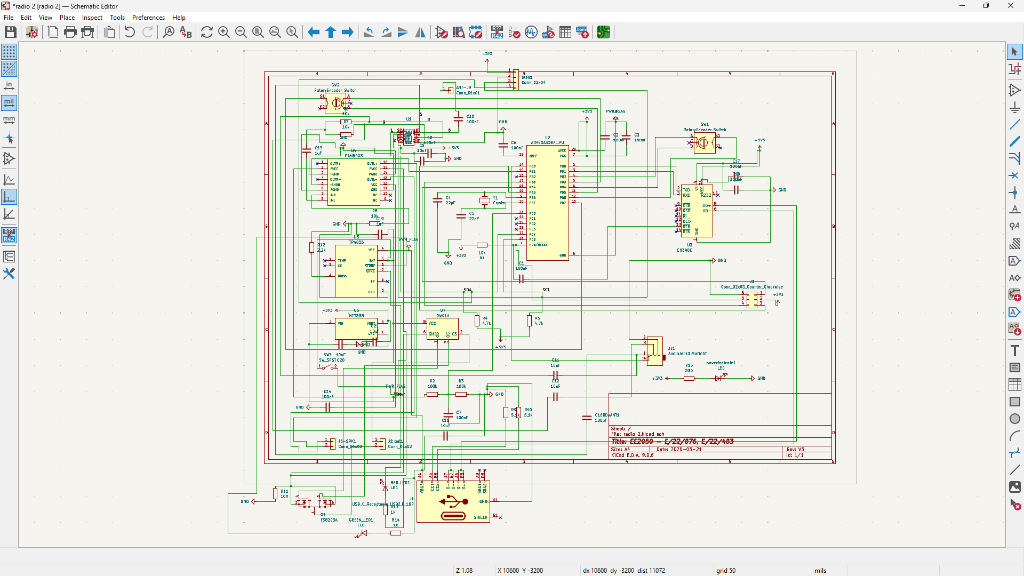
\includegraphics[width=0.9\linewidth]{images/schematic.png}
\caption{Phase~3 KiCad Schematic.}
\label{fig:kicad-schematic}
\end{figure}

\begin{figure}[H]
\centering
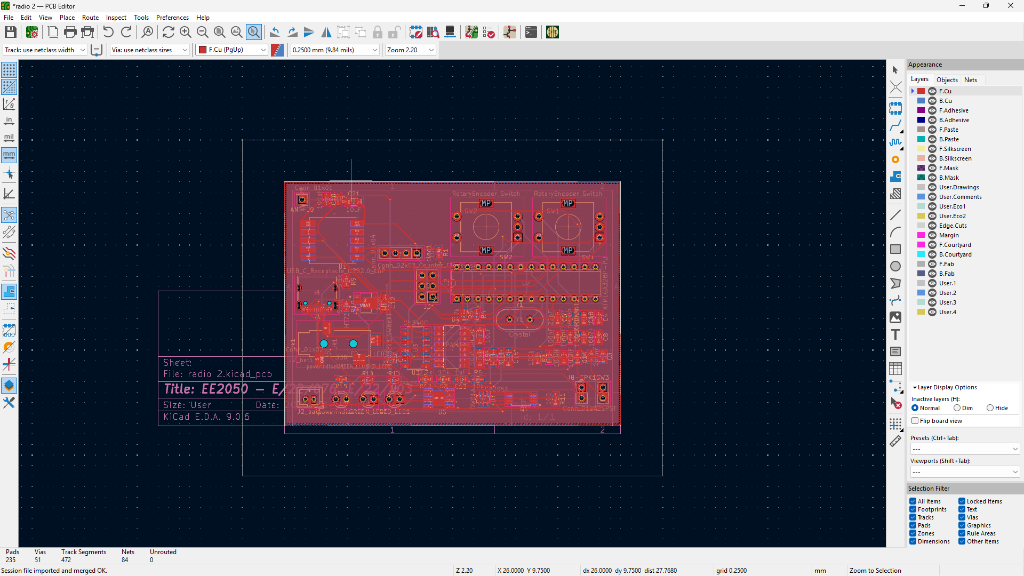
\includegraphics[width=0.9\linewidth]{images/radio2_top.png}
\caption{Phase~3 PCB layout (KiCad PCB Editor) showing fully routed traces.}
\label{fig:pcb-top}
\end{figure}

\begin{figure}[H]
\centering
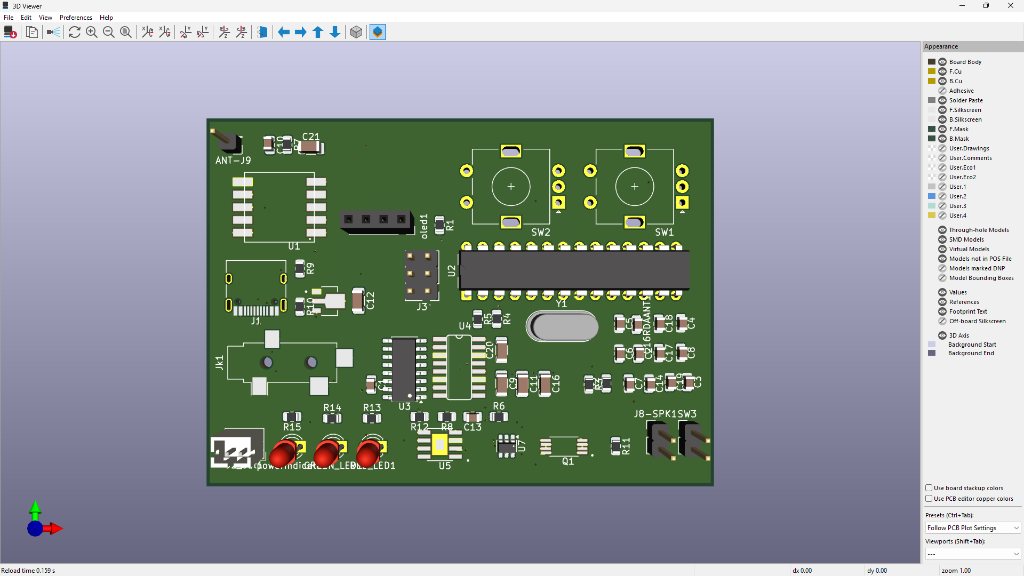
\includegraphics[width=0.9\linewidth]{images/RADIO.png}
\caption{3D render of the PCB (custom component models omitted).}
\label{fig:pcb-3d}
\end{figure}

% ─────────────────────────────────────────────────────────────────────────────
% Part 7 - Challenges, Lessons Learned, Conclusion, and References
% ─────────────────────────────────────────────────────────────────────────────

%% ═══════════════════════════════════════════════════════════════════════════════
\section{Conclusion}
%% ═══════════════════════════════════════════════════════════════════════════════

This project achieved its primary objective - a working FM radio - in
Iteration~1, and progressively enhanced it through two more iterations.  The
final design (Iteration~3) represents a product-grade architecture: custom
PCB, integrated charging, single USB-C port, Class-D amplification, and OLED
display with a 68-station database.  The journey from a noisy perfboard to a
complete PCB design demonstrates the iterative engineering process at its
core.

The Phase~3 design was completed as a software deliverable ready for future
fabrication. No design knowledge has been lost; every decision is traceable.

The AI-assisted methodology proved both powerful and dangerous.  AI models
accelerated the design process dramatically - generating build documents,
debugging hardware issues in real-time, and assisting in comprehensive PCB
verification and DRC review.  But they also introduced errors (wrong IC compatibility
claims, incorrect pinouts in early drafts) that required human verification
against datasheets.  The key lesson: AI is an excellent engineering partner,
but never the final authority.  The engineer must always remain the
decision-maker.

%% ═══════════════════════════════════════════════════════════════════════════════
\section{References}
%% ═══════════════════════════════════════════════════════════════════════════════

\begin{enumerate}[label={[\arabic*]}, nosep, leftmargin=2em]
    \item RDA Microelectronics, ``RDA5807M Single-Chip FM Stereo Radio,''
          Datasheet Rev~1.1, 2011.
    \item Diodes Incorporated, ``PAM8403 3\,W Class-D Audio Amplifier,''
          Datasheet, 2009.
    \item NanJing TopPower, ``TP4056 1\,A Linear Li-Ion Battery Charger,''
          Datasheet, 2006.
    \item Holtek, ``HT7333 Low Dropout Voltage Regulator,'' Datasheet, 2015.
    \item WCH, ``CH340C USB to Serial Interface,'' Datasheet, 2018.
    \item Fortune Semiconductor, ``DW01A One-Cell Li-Ion Battery Protection
          IC,'' Datasheet, 2010.
    \item Fortune Semiconductor, ``FS8205A Dual N-Channel MOSFET,''
          Datasheet, 2010.
    \item Solomon Systech, ``SSD1306 128$\times$64 OLED Driver,'' Datasheet,
          2008.
    \item Microchip, ``ATmega328P 8-bit AVR Microcontroller,'' Datasheet,
          2018.
    \item KiCad EDA, ``KiCad 9.0 Documentation,''
          \url{https://docs.kicad.org}, 2026.
\end{enumerate}


\end{document}
